% =====================================================================
%  CHAPITRE 3 -- partie b : sections 3.2 (fin) et 3.3
% =====================================================================

% ---------------------------------------------------------------- 18
\begin{frame}{HDI : la définition rigoureuse}
\small
\vspace{-1mm}
\begin{kbox}[Densité postérieure la plus élevée (\textit{Highest Density Interval})]
Pour un posterior $p(\theta \given y)$ et un niveau $1-\alpha$, le HDI est
l'ensemble
\[
C_{\text{HDI}} = \big\{\theta : p(\theta \given y) \geq h_{1-\alpha}\big\}
\quad\text{où}\quad h_{1-\alpha} \text{ est le seuil tel que } P(C_{\text{HDI}} \given y) = 1-\alpha .
\]
Conséquence immédiate : \textbf{toute valeur à l'intérieur a une densité
postérieure supérieure à toute valeur à l'extérieur}. C'est donc, parmi tous les
ensembles de masse $1-\alpha$, celui de \textbf{plus petite longueur}.
\end{kbox}
\vspace{1mm}
\begin{columns}[t]
\begin{column}{0.49\textwidth}
\begin{ebox}[Posterior unimodal --- le cas courant]
Le HDI est un intervalle $[a, b]$, solution de
\[
p(a \given y) = p(b \given y) \quad\text{et}\quad \int_a^b p(\theta \given y)\mathrm{d}\theta = 1-\alpha .
\]
Les bornes ont donc \textbf{la même densité} : c'est le test d'arrêt à utiliser
dans un code.
\end{ebox}
\end{column}
\begin{column}{0.49\textwidth}
\begin{wbox}[Posterior multimodal ou à plateau]
Le HDI n'est plus un intervalle : c'est une \textbf{union} de morceaux
(ex. un bimodal donne deux intervalles séparés). Ne jamais dire « le » HDI
sans vérifier l'unimodalité. Un intervalle à queues égales, lui, reste toujours
un intervalle --- mais peut être très large.
\end{wbox}
\end{column}
\end{columns}
\end{frame}

% ---------------------------------------------------------------- 19
\begin{frame}[fragile]{Calculer un HDI : code exact (et version ArviZ)}
\footnotesize
\vspace{-2mm}
\begin{codebox}[Recherche du plus court intervalle de masse $0{,}95$ sur une grille]
\begin{lstlisting}
import numpy as np
from scipy import stats

def hdi_grid(dist, level=0.95, m=200_001):
    x = np.linspace(0.0, float(dist.ppf(1 - 1e-7)), m)
    dens = dist.pdf(x)
    c = np.concatenate([[0.0], np.cumsum((dens[1:] + dens[:-1]) / 2 * np.diff(x))])
    c /= c[-1]                    # fonction de repartition cumulee (trapezes)
    j = np.searchsorted(c, c + level)      # borne droite pour chaque borne gauche
    w = np.where(j < m, x[np.clip(j, 0, m - 1)] - x, np.inf)
    i = int(np.argmin(w))                  # on garde le plus court
    return float(x[i]), float(x[np.clip(j[i], 0, m - 1)])

print(hdi_grid(stats.gamma(a=2.0, scale=2.0)))            # (0.080 ; 9.526)
print(stats.gamma(a=2.0, scale=2.0).ppf([.025, .975]))    # (0.484 ; 11.143)
\end{lstlisting}
\end{codebox}
\vspace{0.5mm}
\begin{columns}[t]
\begin{column}{0.55\textwidth}
\begin{ebox}[Avec ArviZ, sur des tirages MCMC]
\py{az.hdi(draws, hdi_prob=0.95)} renvoie directement les bornes ; c'est
l'équivalent de notre fonction, appliqué à un échantillon au lieu d'une densité
analytique.
\end{ebox}
\end{column}
\begin{column}{0.43\textwidth}
\begin{kbox}[Vérification faite en cours]
Notre fonction donnait $[0{,}484\,;11{,}143]$ à queues égales contre
$[0{,}080\,;9{,}526]$ en HDI pour Gamma$(2\,;0{,}5)$ : $11{,}4\,\%$ de largeur
en moins, calculé, pas supposé.
\end{kbox}
\end{column}
\end{columns}
\end{frame}

% ---------------------------------------------------------------- 20
\begin{frame}{Crédibilité unilatérale : la question du décideur}
\begin{center}
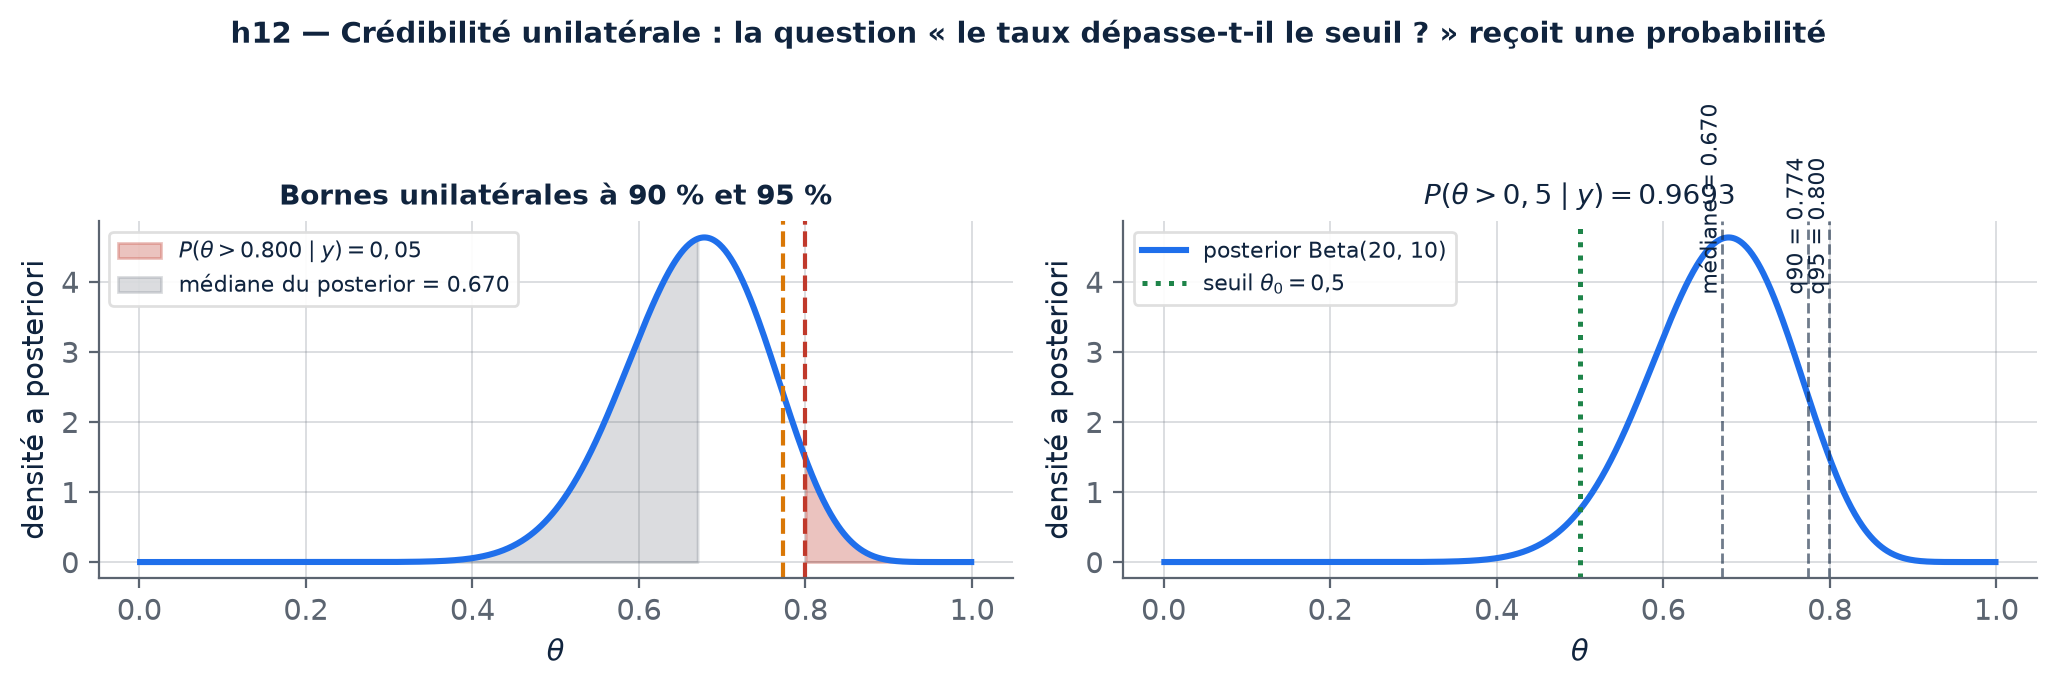
\includegraphics[width=.88\textwidth]{h12_credibilite_unilaterale.png}
\end{center}
\end{frame}

\begin{frame}{Crédibilité unilatérale : la question du décideur}
\small
\begin{columns}[t]
\begin{column}{0.48\textwidth}
\begin{ebox}[Posterior Beta$(20,10)$]
\resizebox{\ifdim\width>\linewidth\linewidth\else\width\fi}{!}{%
\begin{tabular}{@{}lc@{}}
\toprule
Quantile du posterior & valeur \\
\midrule
médiane $q_{0{,}50}$ & $0{,}670$ \\
$q_{0{,}90}$ & $0{,}774$ \\
$q_{0{,}95}$ & $0{,}800$ \\
\bottomrule
\end{tabular}}
\vspace{1.5mm}

$P(\theta > 0{,}5 \given y) = \mathbf{0{,}9693}$
\end{ebox}
\end{column}
\begin{column}{0.48\textwidth}
\begin{solbox}[Trois phrases possibles]
\footnotesize
\begin{itemize}
  \item « au moins $50\,\%$ de chance que $\theta > 0{,}670$ » ;
  \item « le taux dépasse $0{,}5$ à $96{,}9\,\%$ de probabilité » ;
  \item « borne supérieure à $90\,\%$ : $0{,}774$ ».
\end{itemize}
\end{solbox}
\end{column}
\end{columns}
\vspace{1mm}
\begin{kbox}[Unilatéral contre bilatéral]
$[q_{0{,}05} ; +\infty[$ et $]-\infty ; q_{0{,}95}]$ ont chacun $95\,\%$ de masse,
mais ils ne répondent pas à la même question. Le décideur veut presque toujours
un \textbf{unilatéral} (« est-ce au-dessus du seuil ? »), le statisticien publie
souvent un bilatéral par habitude.
\end{kbox}
\end{frame}

% ---------------------------------------------------------------- 21
\begin{frame}{Quiz --- Intervalles : le bon outil au bon moment}
\begin{qbox}[Quatre situations, quatre intervalles]
Pour chaque cas, choisissez l'outil correct et justifiez en une ligne.
\vspace{1mm}
\begin{enumerate}
  \item[(1)] Posterior Beta$(0{,}5, 0{,}5)$ très asymétrique : on veut « l'intervalle
        à $95\,\%$ » pour un graphique de synthèse.
  \item[(2)] Le régulateur demande : « le taux de défaut est-il \emph{sous} $2\,\%$ ? »
  \item[(3)] On publie un tableau comparatif avec des IC fréquentistes :
        on veut la comparaison la moins biaisée possible.
  \item[(4)] Posterior bimodal (mélange de deux populations) : on veut
        « l'intervalle à $95\,\%$ ».
\end{enumerate}
\vspace{1mm}
\textbf{Réponses :} (1) HDI, nettement plus court ; (2) \textbf{unilatéral}
$]-\infty\,;q_{0{,}95}]$ avec la probabilité annoncée ; (3) queues égales
(identique à l'IC quand le prior est plat) ; (4) \textbf{aucun intervalle unique} :
il faut publier l'union des deux morceaux, ou traiter les deux sous-populations
séparément.
\end{qbox}
\end{frame}

% ---------------------------------------------------------------- 22
\begin{frame}{Tableau comparatif : IC fréquentiste contre intervalle crédible}
\small
\vspace{-2mm}
\begin{center}
{\footnotesize
\begin{tabular}{@{}p{0.14\textwidth}p{0.34\textwidth}p{0.40\textwidth}@{}}
\toprule
\textbf{Critère} & \textbf{Intervalle de confiance (fréquentiste)} & \textbf{Intervalle de crédibilité (bayésien)} \\
\midrule
Objet aléatoire & l'\textbf{intervalle} (les données changent) & le \textbf{paramètre} $\theta$ \\
\addlinespace
Énoncé correct & « $95\,\%$ des intervalles ainsi construits contiennent $\theta$ » &
$P(\theta \in [a,b] \given y) = 0{,}95$ \\
\addlinespace
Énoncé incorrect & « \nok{} il y a $95\,\%$ de chance que $\theta$ soit dedans » &
« \nok{} $95\,\%$ des répétitions contiendront $\theta$ » \\
\addlinespace
Dépend du prior & non & \warn{} oui, explicitement \\
\addlinespace
Peut être asymétrique & rarement (transformations) & oui, et c'est un choix \\
\addlinespace
Interprétation métier & « précision de la méthode » &
« croyance actuelle sur la valeur » \\
\addlinespace
Avec $n$ grand, prior plat & référence & \ok{} coïncide numériquement \\
\bottomrule
\end{tabular}}
\end{center}
\vspace{1mm}
\begin{wbox}[La phrase à ne jamais prononcer]
\nok{} « Il y a $95\,\%$ de chance que la vraie valeur soit dans \emph{cet}
intervalle de confiance. » Un IC fréquentiste, une fois calculé, contient $\theta$
ou ne le contient pas : la probabilité est $0$ ou $1$. Seul l'intervalle
\emph{crédible} porte une probabilité sur $\theta$.
\end{wbox}
\end{frame}

% ---------------------------------------------------------------- 23
\begin{frame}{La garantie se mesure : couverture empirique sur 2\,000 échantillons}
\begin{center}
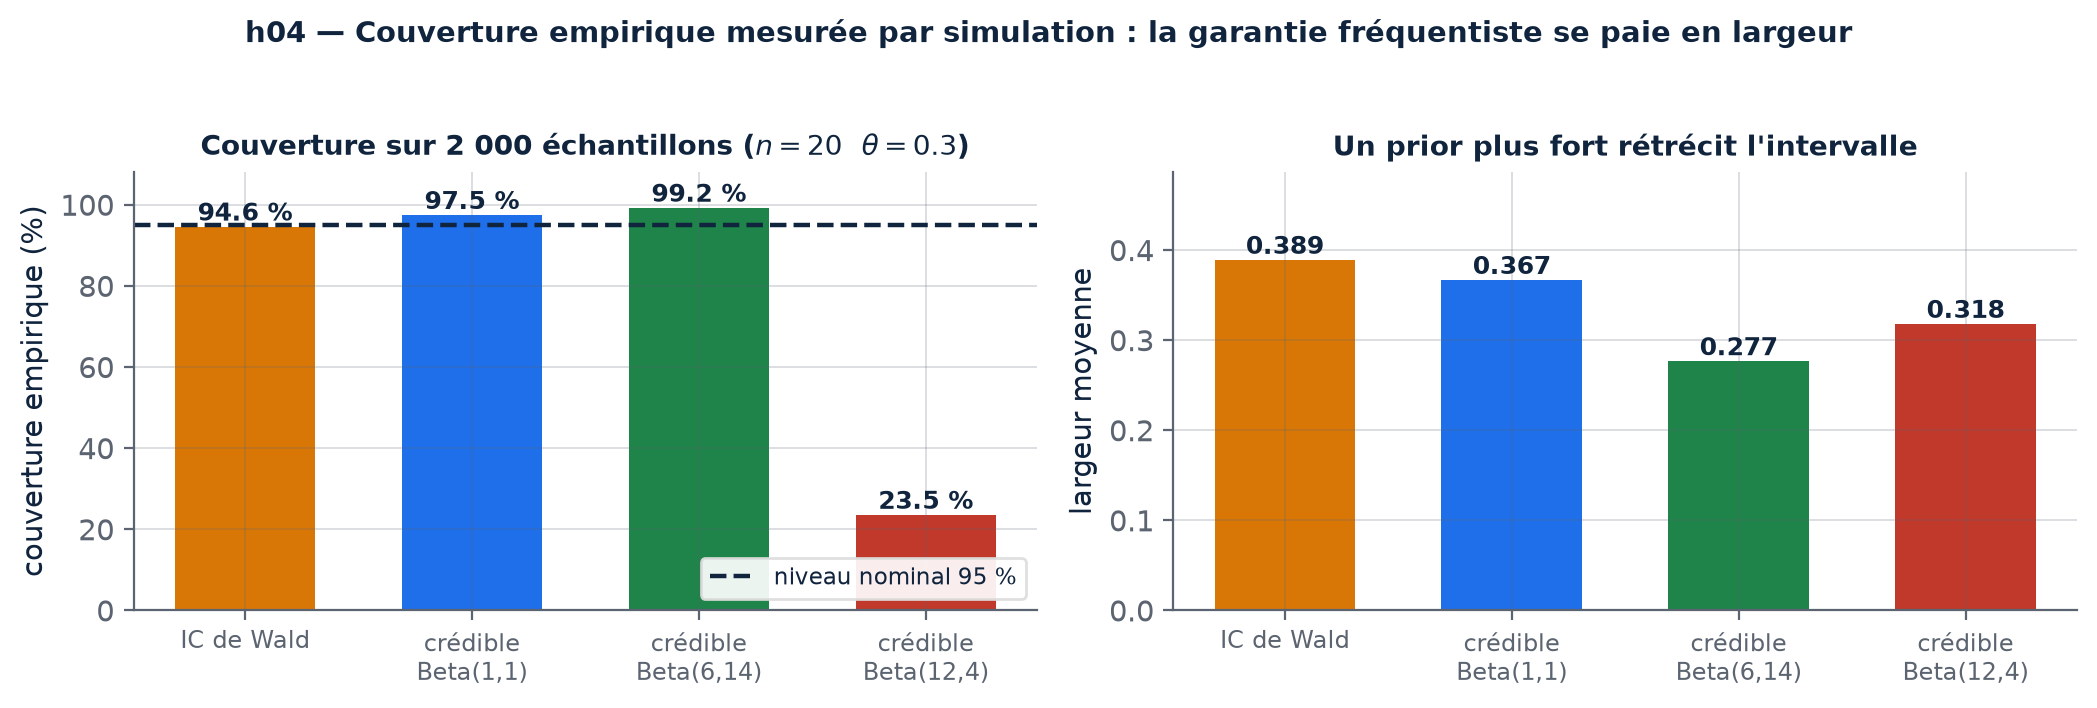
\includegraphics[width=.95\textwidth]{h04_couverture.png}
\end{center}
\vspace{-1.5mm}
\begin{columns}[t]
\begin{column}{0.60\textwidth}
\begin{ebox}[Protocole réellement exécuté]
$\theta_{\text{vrai}} = 0{,}30$, $n = 20$, \textbf{2\,000 échantillons} simulés
($k \sim \mathrm{Bin}(20 ; 0{,}30)$). Pour chacun, on calcule quatre intervalles à
$95\,\%$ et on teste s'ils contiennent $\theta_{\text{vrai}}$. On obtient la
fréquence de couverture --- la seule preuve honnête qu'un intervalle tient sa
promesse.
\end{ebox}
\end{column}
\begin{column}{0.38\textwidth}
\begin{solbox}[Couverture mesurée]
\small
\resizebox{\ifdim\width>\linewidth\linewidth\else\width\fi}{!}{%
\begin{tabular}{@{}lc@{}}
\toprule
Méthode & couverture \\
\midrule
IC de Wald & $94{,}6\,\%$ \\
crédible, prior Beta$(1,1)$ & $97{,}5\,\%$ \\
crédible, prior Beta$(6,14)$ & $99{,}3\,\%$ \\
crédible, prior Beta$(12,4)$ & \textcolor{byRed}{$23{,}6\,\%$} \\
\bottomrule
\end{tabular}}
\end{solbox}
\end{column}
\end{columns}
\end{frame}

% ---------------------------------------------------------------- 24
\begin{frame}{Ce que la couverture révèle (et ce qu'elle cache)}
\begin{columns}[t]
\begin{column}{0.49\textwidth}
\begin{ebox}[Lire le second panneau]
\begin{tabular}{@{}lcc@{}}
\toprule
Méthode & couverture & largeur moyenne \\
\midrule
IC de Wald & $94{,}6\,\%$ & $0{,}3891$ \\
Beta$(1,1)$ & $97{,}5\,\%$ & $0{,}3667$ \\
Beta$(6,14)$ & $99{,}3\,\%$ & $0{,}2766$ \\
Beta$(12,4)$ & $23{,}6\,\%$ & $0{,}3180$ \\
\bottomrule
\end{tabular}
\vspace{1.5mm}

\small Le prior \textbf{correct} (Beta$(6,14)$, centré sur $0{,}30$) rétrécit
l'intervalle de $29\,\%$ \emph{et} augmente la couverture : c'est le gain
authentique de l'information externe.
\end{ebox}
\end{column}
\begin{column}{0.49\textwidth}
\begin{wbox}[Le revers de la médaille]
Le prior Beta$(12,4)$ est centré sur $0{,}75$ alors que $\theta = 0{,}30$ :
l'intervalle crédible ne couvre la vérité que dans $23{,}6\,\%$ des cas
\emph{malgré} son étiquette « $95\,\%$ ». Un prior faux ne se contente pas de
rétrécir : il \textbf{ment avec assurance}.
\end{wbox}
\begin{kbox}[La règle d'or]
La garantie bayésienne est \textbf{conditionnelle au prior}. Sur des données
abondantes, tout prior raisonnable converge ; sur de petites données, la
couverture mesurée est l'outil de diagnostic obligatoire --- et elle se calcule.
\end{kbox}
\end{column}
\end{columns}
\end{frame}

% ---------------------------------------------------------------- 25
\begin{frame}{Activité --- Mesurez la couverture vous-mêmes (10 min)}
\begin{abox}[Protocole à coder en binôme]
\begin{enumerate}
  \item Simulez 2\,000 jeux de données : $k = $ \py{rng.binomial(20, 0.3, 2000)}.
  \item Pour chaque jeu, calculez l'IC de Wald
        $\hat p \pm 1{,}96\sqrt{\hat p(1-\hat p)/n}$.
  \item Puis l'intervalle crédible Beta$(1+k,\,1+n-k)$ (queues égales).
  \item Estimez la couverture : \py{np.mean((lo <= 0.3) & (0.3 <= hi))}.
  \item Recommencez avec $n = 5$, puis $n = 100$. Que devient la divergence entre
        les deux méthodes ?
\end{enumerate}
\end{abox}
\vspace{1mm}
\begin{columns}[t]
\begin{column}{0.49\textwidth}
\begin{solbox}[Résultats de référence ($n = 20$)]
Wald $94{,}6\,\%$ ; crédible Beta$(1,1)$ $97{,}5\,\%$.
L'IC de Wald \emph{sous}-couvre légèrement : c'est l'approximation normale, qui
néglige l'asymétrie du posterior à petit $n$.
\end{solbox}
\end{column}
\begin{column}{0.49\textwidth}
\begin{kbox}[Ce qu'il faut voir]
Aux petits $n$, le crédible à prior plat couvre \textbf{mieux} que l'IC classique :
la loi a posteriori exacte remplace une approximation asymptotique. C'est un
argument de robustesse, indépendant de tout a priori subjectif.
\end{kbox}
\end{column}
\end{columns}
\end{frame}

% ---------------------------------------------------------------- 26
\begin{frame}{Synthèse de la section 3.2 --- cinq règles}
\small
\vspace{-1mm}
\begin{columns}[t]
\begin{column}{0.49\textwidth}
\begin{kbox}[Les cinq règles]
\begin{enumerate}
  \item Toujours dire \textbf{quel} intervalle (queues égales, HDI, unilatéral).
  \item Sur un posterior asymétrique, préférer le \textbf{HDI}
        (jusqu'à $14\,\%$ plus court à masse égale).
  \item Pour une décision à seuil, publier un \textbf{unilatéral} et la
        probabilité $P(\theta > \theta_0 \given y)$.
  \item Ne jamais attribuer une probabilité à un IC fréquentiste.
  \item \textbf{Mesurer} la couverture par simulation avant de s'engager.
\end{enumerate}
\end{kbox}
\end{column}
\begin{column}{0.49\textwidth}
\begin{ebox}[Les chiffres de la section]
\resizebox{\ifdim\width>\linewidth\linewidth\else\width\fi}{!}{%
\begin{tabular}{@{}ll@{}}
\toprule
HDI sur Gamma$(2\,;0{,}5)$ & gain $11{,}4\,\%$ \\
HDI sur $\chi^2_3$ & gain $14{,}4\,\%$ \\
Couverture IC de Wald & $94{,}6\,\%$ \\
Couverture crédible Beta$(1,1)$ & $97{,}5\,\%$ \\
Couverture avec prior faux & $23{,}6\,\%$ \\
$P(\theta > 0{,}5)$ sur Beta$(20,10)$ & $0{,}9693$ \\
\bottomrule
\end{tabular}}
\vspace{1.5mm}
\tiny Toutes ces valeurs sortent de \file{src/fig\_ch3.py}, exécuté pour ce cours.
\end{ebox}
\end{column}
\end{columns}
\vspace{1mm}
\begin{tcolorbox}[colback=byCyan!8,colframe=byCyan,arc=2mm,width=.96\textwidth]
\centering\small
\textbf{Bascule vers 3.3} : un intervalle décrit $\theta$ ; le décideur, lui, veut
souvent \emph{la prochaine observation}. Ce n'est pas la même loi --- et c'est plus large.
\end{tcolorbox}
\end{frame}

% ---------------------------------------------------------------- 27
\begin{frame}{Section 3.3 --- Prédire : la loi prédictive a posteriori}
\small
\vspace{-1.5mm}
\begin{kbox}[Définition --- prédictive a posteriori]
\[
p(\tilde y \given y) \;=\; \int p(\tilde y \given \theta)\, p(\theta \given y)\, \mathrm{d}\theta .
\]
On \textbf{moyenne la vraisemblance de la nouvelle observation sur tout le
posterior} : on propage donc deux incertitudes --- celle du modèle
($p(\tilde y \given \theta)$) et celle du paramètre ($p(\theta \given y)$).
\end{kbox}
\vspace{1mm}
\begin{columns}[t]
\begin{column}{0.49\textwidth}
\begin{ebox}[Trois propriétés à connaître]
\begin{itemize}
  \item La prédictive est \textbf{toujours plus large} que la vraisemblance
        évaluée au point estimé : ignorer l'incertitude sur $\theta$, c'est
        sous-estimer le risque.
  \item Pour les couples conjugués, elle a une forme close
        (Beta-Binomial, Gamma-Poisson, Normal-Normal).
  \item Sans forme close, on l'approxime par \textbf{Monte-Carlo} :
        tirer $\theta^{(s)} \sim p(\theta \given y)$, puis
        $\tilde y^{(s)} \sim p(\tilde y \given \theta^{(s)})$.
\end{itemize}
\end{ebox}
\end{column}
\begin{column}{0.49\textwidth}
\begin{wbox}[Erreur classique]
\small Brancher le \emph{point estimate} dans le modèle et présenter la sortie
comme une prédiction : c'est ignorer $\Var(\theta \given y)$. L'intervalle obtenu
est trop étroit, donc \textbf{dangereux} (stocks, capacités, garanties). Pour
prédire, il faut la prédictive, pas la vraisemblance au mode.
\end{wbox}
\end{column}
\end{columns}
\end{frame}

% ---------------------------------------------------------------- 28
\begin{frame}{Prédiction a posteriori : le cas des accidents}
\small
\vspace{-2.5mm}
\begin{center}
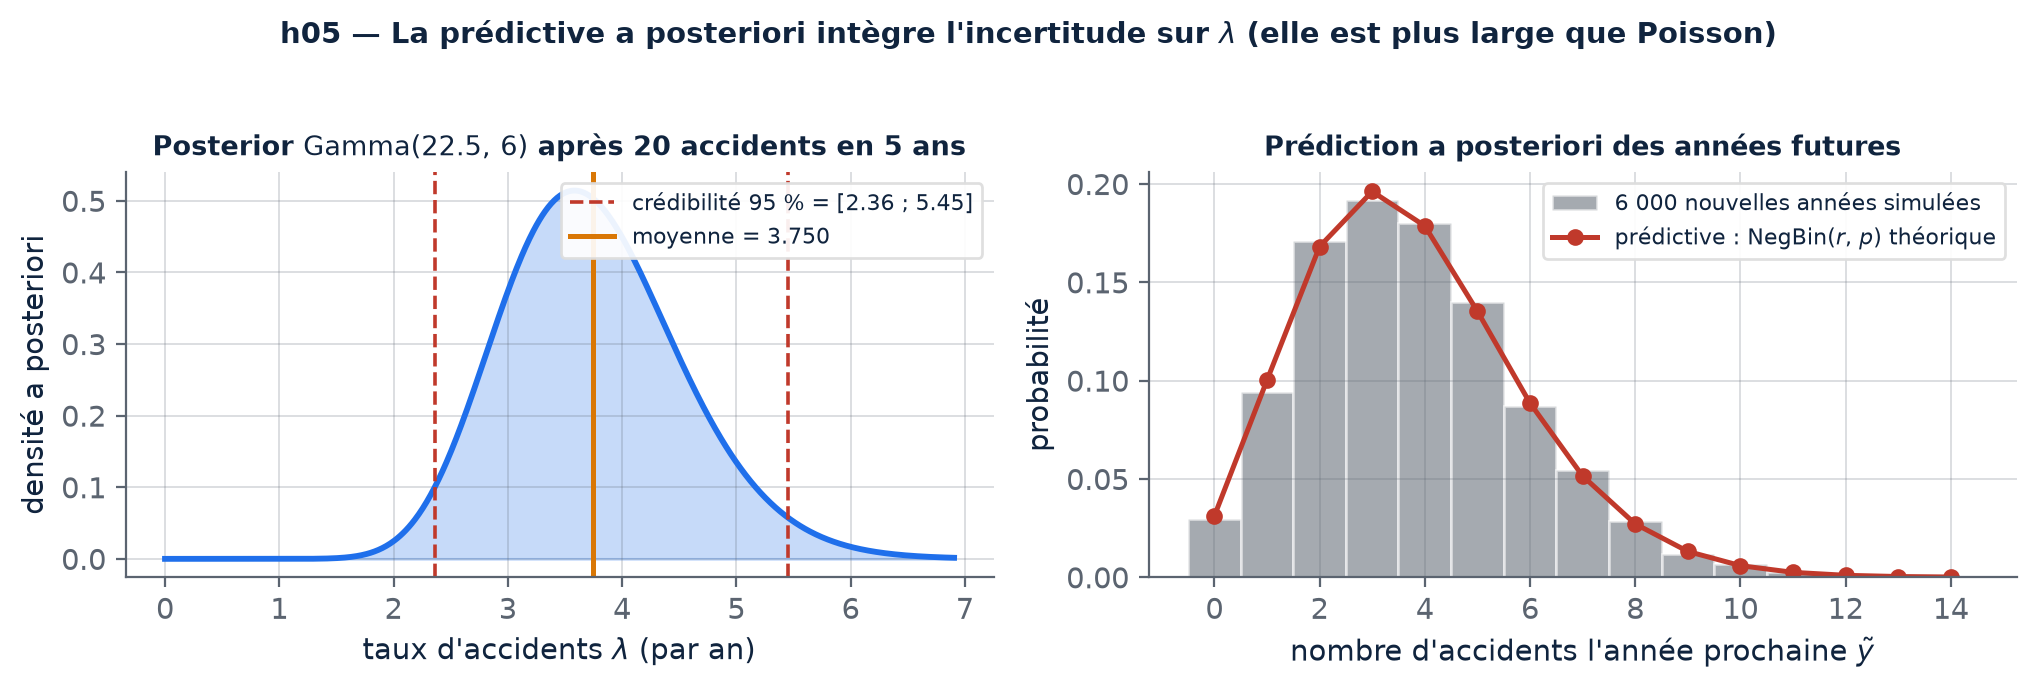
\includegraphics[width=.80\textwidth]{h05_predictive.png}
\end{center}
\vspace{-1.5mm}
\begin{columns}[t]
\begin{column}{0.55\textwidth}
\begin{ebox}[Données et posterior]
Un site a connu $4, 2, 5, 3, 6$ accidents sur cinq années, soit
\textbf{20 accidents} au total. Prior Gamma$(2{,}5\,;1)$ sur le taux annuel
$\lambda$ ; vraisemblance de Poisson.
\[
\lambda \given y \sim \mathrm{Gamma}(2{,}5 + 20 \,;\, 1 + 5)
= \mathrm{Gamma}(22{,}5\,;\,6)
\]
moyenne $3{,}75$ accidents par an, crédibilité $95\,\%$
$[2{,}36\,;5{,}45]$.
\end{ebox}
\end{column}
\begin{column}{0.43\textwidth}
\begin{solbox}[Lecture du gestionnaire]
\begin{itemize}
  \item $P(\lambda > 4 \given y) = 0{,}352$ : \warn{} un risque réel
        d'être au-dessus du seuil de $4$.
  \item $P(\tilde y > 6 \given y) = 0{,}102$ pour l'année prochaine.
  \item La probabilité d'une année \emph{sans} accident : $2{,}95\,\%$
        (simulation).
\end{itemize}
\end{solbox}
\end{column}
\end{columns}
\end{frame}

% ---------------------------------------------------------------- 29
\begin{frame}[fragile]{La prédictive sans formule : Monte-Carlo}
\begin{codebox}[Deux lignes de simulation, et la forme close pour vérifier]
\begin{lstlisting}
from scipy import stats
import numpy as np

obs = np.array([4, 2, 5, 3, 6])                 # 5 annees d'historique
a_post, b_post = 2.5 + obs.sum(), 1 + len(obs)  # posterior Gamma(22.5 ; 6)  [taux 6]
post = stats.gamma(a_post, scale=1 / b_post)

# --- predictive par Monte-Carlo (aucune formule necessaire) -----------------
lam_draws = post.rvs(20_000, random_state=4112)
y_new = np.random.default_rng(4112).poisson(lam_draws)

print(lam_draws.mean())                          # 3.75   moyenne a posteriori de lambda
print(np.percentile(lam_draws, [2.5, 97.5]))     # [2.36 ; 5.45]  credibilite 95 %
print(np.mean(y_new > 6))                        # 0.102  annee prochaine > 6 accidents
print(np.mean(y_new == 0))                       # 0.030  annee sans aucun accident

# --- verification par la forme close : Gamma-Poisson -> binomiale negative --
nb = stats.nbinom(a_post, b_post / (b_post + 1))
print(nb.sf(6))                                  # 0.1018 : accord a 1e-3 pres
\end{lstlisting}
\end{codebox}
\vspace{0mm}
\centering\footnotesize
Le Monte-Carlo et la formule exacte donnent la même réponse : c'est la
vérification croisée qui valide l'échantillonneur. Sorties réellement obtenues :
$3{,}75$, $[2{,}36\,;5{,}45]$, $0{,}102$, $0{,}030$, $0{,}1018$.
\end{frame}

% ---------------------------------------------------------------- 30
\begin{frame}{Posterior predictive check : le modèle sait-il reproduire les données ?}
\small
\vspace{-3mm}
\begin{center}
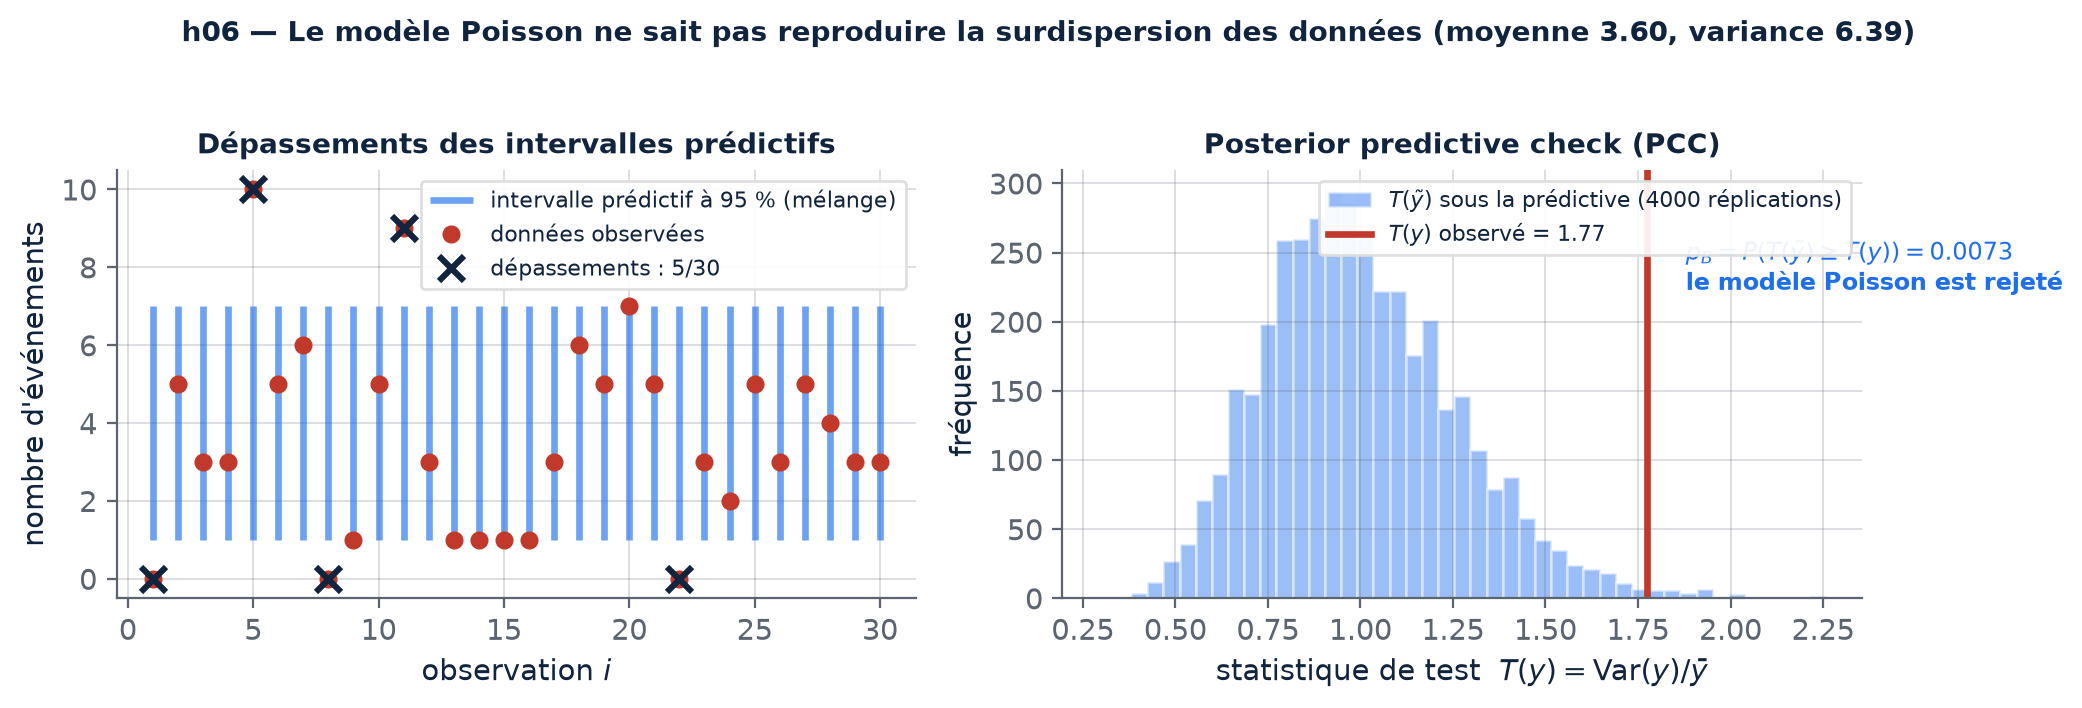
\includegraphics[width=.74\textwidth]{h06_ppc.png}
\end{center}
\vspace{-1.5mm}
\begin{columns}[t]
\begin{column}{0.55\textwidth}
\begin{ebox}[Protocole (Box, 1980)]
\begin{enumerate}
  \item Choisir une \textbf{statistique de test} $T(y)$ qui cible le défaut
        suspecté (ici la surdispersion : $T = \Var(y)/\bar y$).
  \item Tirer $\theta^{(s)} \sim p(\theta \given y)$ puis
        $\tilde y^{(s)} \sim p(\tilde y \given \theta^{(s)})$.
  \item Calculer la \textbf{probabilité a posteriori de queue}
        $p_B = P\big(T(\tilde y) \geq T(y) \given y\big)$.
\end{enumerate}
\end{ebox}
\end{column}
\begin{column}{0.43\textwidth}
\begin{solbox}[Résultat mesuré]
\begin{itemize}
  \item $T(y) = \Var(y)/\bar y = 1{,}774$ (moyenne $3{,}60$,
        variance $6{,}39$).
  \item $\mathbf{p_B = 0{,}0073}$ sur 4\,000 réplications.
  \item Depassements des intervalles prédictifs : $5/30$.
\end{itemize}
\vspace{1mm}
\footnotesize Conclusion : le modèle de Poisson \textbf{est rejeté}
(surdispersion).
\end{solbox}
\end{column}
\end{columns}
\end{frame}

% ---------------------------------------------------------------- 31
\begin{frame}{Lire un \textit{posterior predictive check} correctement}
\begin{columns}[t]
\begin{column}{0.49\textwidth}
\begin{kbox}[Ce que $p_B$ n'est pas]
\begin{itemize}
  \item \textbf{Pas} une $p$-value fréquentiste : c'est une probabilité a
        posteriori calculée \emph{sous le modèle}, sans hypothèse nulle.
  \item \textbf{Pas} une preuve de validité : un $p_B$ central ($\approx 0{,}5$)
        signifie seulement que la statistique choisie ne détecte rien.
  \item \textbf{Pas} un test de « vérité » du modèle : tous les modèles sont faux,
        certains sont utiles.
\end{itemize}
\end{kbox}
\end{column}
\begin{column}{0.49\textwidth}
\begin{ebox}[Ce $p_B$ dit vraiment]
Le modèle postule $\Var(y) = \E[y]$ (Poisson). Or la statistique observée
$1{,}774$ est plus grande que dans $99{,}3\,\%$ des réplications simulées.
Autrement dit : \textbf{même en tirant au hasard sous ce modèle, on n'obtient
presque jamais une variabilité aussi forte}. Il faut passer à une
binomiale négative (ou un modèle hiérarchique).
\end{ebox}
\end{column}
\end{columns}
\vspace{1mm}
\begin{wbox}[Le piège du dépassement isolé]
$5$ observations sur $30$ sortent de l'intervalle prédictif à $95\,\%$ : c'est
$16{,}7\,\%$ au lieu de $5\,\%$ attendus. Un dépassement ponctuel n'est pas
grave ; $5$ sur $30$ \textbf{avec} $p_B = 0{,}0073$, c'est un signal.
\end{wbox}
\end{frame}

% ---------------------------------------------------------------- 32
\begin{frame}{Activité --- Écrire un PPC de A à Z (12 min)}
\begin{abox}[Consigne]
On dispose du posterior du taux d'accidents $\mathrm{Gamma}(22{,}5\,;6)$ et du
modèle de Poisson.
\begin{enumerate}
  \item Choisissez \textbf{deux} statistiques de test : le maximum observé, et la
        proportion de valeurs nulles.
  \item Simulez $5\,000$ jeux de données de taille $n = 30$.
  \item Calculez $p_B$ pour chaque statistique.
  \item Conclusion : le modèle de Poisson est-il adapté aux données du site ?
\end{enumerate}
\end{abox}
\vspace{1mm}
\begin{columns}[t]
\begin{column}{0.49\textwidth}
\begin{solbox}[Résultats du cours, mêmes données]
$T = \Var(y)/\bar y$ : $T(y) = 1{,}774$ et $p_B = 0{,}0073$.
Les deux statistiques proposées ici explorent la même surdispersion sous un
autre angle.
\end{solbox}
\end{column}
\begin{column}{0.49\textwidth}
\begin{kbox}[Le réflexe professionnel]
Un PPC coûte dix lignes de code et évite des mois de conclusions fausses. Dans un
rapport, il se présente \textbf{avant} les résultats : « voici pourquoi ce modèle
est une description défendable de ces données ».
\end{kbox}
\end{column}
\end{columns}
\end{frame}

% ---------------------------------------------------------------- 33
\begin{frame}{Quiz --- Prédiction : les trois pièges}
\begin{qbox}[Question --- Le piège du point estimé]
Un ingénieur calcule $\E[\lambda \given y] = 3{,}75$ puis annonce : « l'année
prochaine, il y aura entre $3{,}75 \pm 1{,}96\sqrt{3{,}75}$, soit
$[0{,}05\,;7{,}45]$ accidents ». Qu'y a-t-il de faux ?
\vspace{1.5mm}
\begin{enumerate}
  \item[(A)] Rien : c'est l'intervalle de Poisson au point estimé.
  \item[(B)] L'intervalle ignore l'incertitude sur $\lambda$ : il est
        \textbf{trop étroit}.
  \item[(C)] L'intervalle est trop large.
  \item[(D)] Il faudrait utiliser la médiane.
\end{enumerate}
\vspace{1mm}
\textbf{Réponse : (B).} La prédictive exacte (binomiale négative) donne
$P(\tilde y > 6) = 0{,}1018$, à comparer à la vraisemblance au point estimé. La
bonne pratique : propager l'incertitude sur $\lambda$ --- deux lignes de
Monte-Carlo suffisent, et la prédictive est \textbf{nécessairement plus large}
que la vraisemblance au point estimé.
\end{qbox}
\end{frame}

% ---------------------------------------------------------------- 34
\begin{frame}{Synthèse de la section 3.3}
\begin{center}
{\small
\begin{tabular}{@{}p{0.15\textwidth}p{0.31\textwidth}p{0.36\textwidth}@{}}
\toprule
\textbf{Objet} & \textbf{Définition} & \textbf{Usage} \\
\midrule
Posterior $p(\theta \given y)$ & croyance sur le paramètre &
décrire, comparer, décider sur $\theta$ \\
\addlinespace
Prédictive $p(\tilde y \given y)$ & moyenne de la vraisemblance sous le posterior &
dimensionner, anticiper, budgéter \\
\addlinespace
Prédictive \textit{joint} $p(\tilde{\mathbf y} \given y)$ & loi du \emph{vecteur}
des observations futures & valider le modèle (PPC), détecter les dépendances \\
\bottomrule
\end{tabular}}
\end{center}
\vspace{1.5mm}
\begin{columns}[t]
\begin{column}{0.49\textwidth}
\begin{kbox}[À retenir]
La prédictive est \textbf{toujours plus large} que l'intervalle au point estimé.
En dimensionner une capacité sans propager l'incertitude sur les paramètres,
c'est se donner une fausse assurance.
\end{kbox}
\end{column}
\begin{column}{0.49\textwidth}
\begin{ebox}[Les chiffres de la section]
Gamma$(22{,}5\,;6)$ : moyenne $3{,}75$, crédibilité $[2{,}36\,;5{,}45]$.
$P(\tilde y > 6 \given y) = 0{,}1018$ (forme close) contre $0{,}102$
(Monte-Carlo). PPC sur la surdispersion : $p_B = 0{,}0073$, rejet du Poisson.
\end{ebox}
\end{column}
\end{columns}
\end{frame}
